\documentclass[tikz,border=0pt]{standalone}
\usepackage{fontspec}
\setmainfont{TeX Gyre Heros}
\setsansfont{TeX Gyre Heros}
\usepackage{amssymb}
\usetikzlibrary{arrows.meta,positioning,calc}
% Shared visual language for Cosmon diagrams. Included after tikz is loaded.
\ifdefined\lightmode
  \definecolor{CosmonBg}{HTML}{E8EFE7}
  \definecolor{CosmonInk}{HTML}{172019}
  \definecolor{CosmonMuted}{HTML}{59665B}
  \definecolor{CosmonFaint}{HTML}{AAB7AA}
  \definecolor{CosmonPanel}{HTML}{F4F7F2}
  \definecolor{CosmonAccent}{HTML}{176D2B}
\else
  \definecolor{CosmonBg}{HTML}{08090C}
  \definecolor{CosmonInk}{HTML}{E7E9E7}
  \definecolor{CosmonMuted}{HTML}{969D97}
  \definecolor{CosmonFaint}{HTML}{444A45}
  \definecolor{CosmonPanel}{HTML}{101317}
  \definecolor{CosmonAccent}{HTML}{3FB950}
\fi

\colorlet{CosmonRoadmap}{CosmonMuted}

\tikzset{
  cosmon text/.style={font=\sffamily\color{CosmonInk}},
  cosmon micro/.style={font=\sffamily\fontsize{6.4}{7.7}\selectfont, text=CosmonMuted},
  cosmon small/.style={font=\sffamily\fontsize{7.4}{9}\selectfont, text=CosmonInk},
  cosmon label/.style={font=\sffamily\bfseries\fontsize{7.2}{8.6}\selectfont, text=CosmonMuted},
  cosmon title/.style={font=\sffamily\bfseries\fontsize{11}{13}\selectfont, text=CosmonInk},
  cosmon frame/.style={draw=CosmonFaint, line width=.55pt, rounded corners=4pt},
  cosmon panel/.style={draw=CosmonFaint, fill=CosmonPanel, line width=.45pt, rounded corners=3pt},
  cosmon molecule/.style={circle, fill=CosmonInk, minimum size=3.6pt, inner sep=0pt},
  cosmon dependency/.style={draw=CosmonMuted, line width=.5pt, -{Latex[length=2.5pt,width=2.1pt]}},
  cosmon data/.style={draw=CosmonInk, line width=1.6pt, {Latex[length=3.1pt,width=2.5pt]}-{Latex[length=3.1pt,width=2.5pt]}},
  cosmon outbound/.style={draw=CosmonAccent, line width=1.05pt, -{Latex[length=3.4pt,width=2.8pt]}},
  cosmon exchange/.style={draw=CosmonInk, line width=.75pt, {Latex[length=3pt,width=2.4pt]}-{Latex[length=3pt,width=2.4pt]}},
  cosmon roadmap/.style={draw=CosmonRoadmap, line width=.65pt, dashed, dash pattern=on 2.4pt off 2.2pt},
  cosmon roadmap arrow/.style={cosmon roadmap, {Latex[length=2.7pt,width=2.2pt]}-{Latex[length=2.7pt,width=2.2pt]}},
  cosmon slot/.style={draw=CosmonAccent, line width=1.2pt, rounded corners=.7pt},
  cosmon peer/.style={circle, draw=CosmonRoadmap, dashed, line width=.6pt, minimum size=13pt, inner sep=0pt},
}

% Canonical glyphs: use these in both diagrams and in the generated legend.
\newcommand{\PilotGlyph}{\textcolor{CosmonAccent}{\ensuremath{\blacklozenge}}}
\newcommand{\MoleculeGlyph}{\textcolor{CosmonInk}{\ensuremath{\bullet}}}
\newcommand{\TraceGlyph}{\textcolor{CosmonAccent}{\ensuremath{\therefore}}}

% The detailed figure's one and only legend, built from the same styles as the art.
\newcommand{\CosmonLegend}{%
  \begin{scope}[shift={(0,0)}]
    \draw[cosmon dependency] (.60,.30) -- (1.22,.30);
    \node[cosmon micro, anchor=west] at (1.36,.30) {thin = ordering dependency};
    \draw[cosmon data] (4.38,.30) -- (5.00,.30);
    \node[cosmon micro, anchor=west] at (5.14,.30) {thick = content in shared files};
    \draw[cosmon roadmap] (8.83,.30) -- (9.45,.30);
    \node[cosmon micro, anchor=west] at (9.59,.30) {dashed = roadmap};
    \node[cosmon micro, anchor=west] at (11.82,.30)
      {\PilotGlyph\ pilot\quad \MoleculeGlyph\ molecule\quad \TraceGlyph\ durable trace};
  \end{scope}%
}


\begin{document}
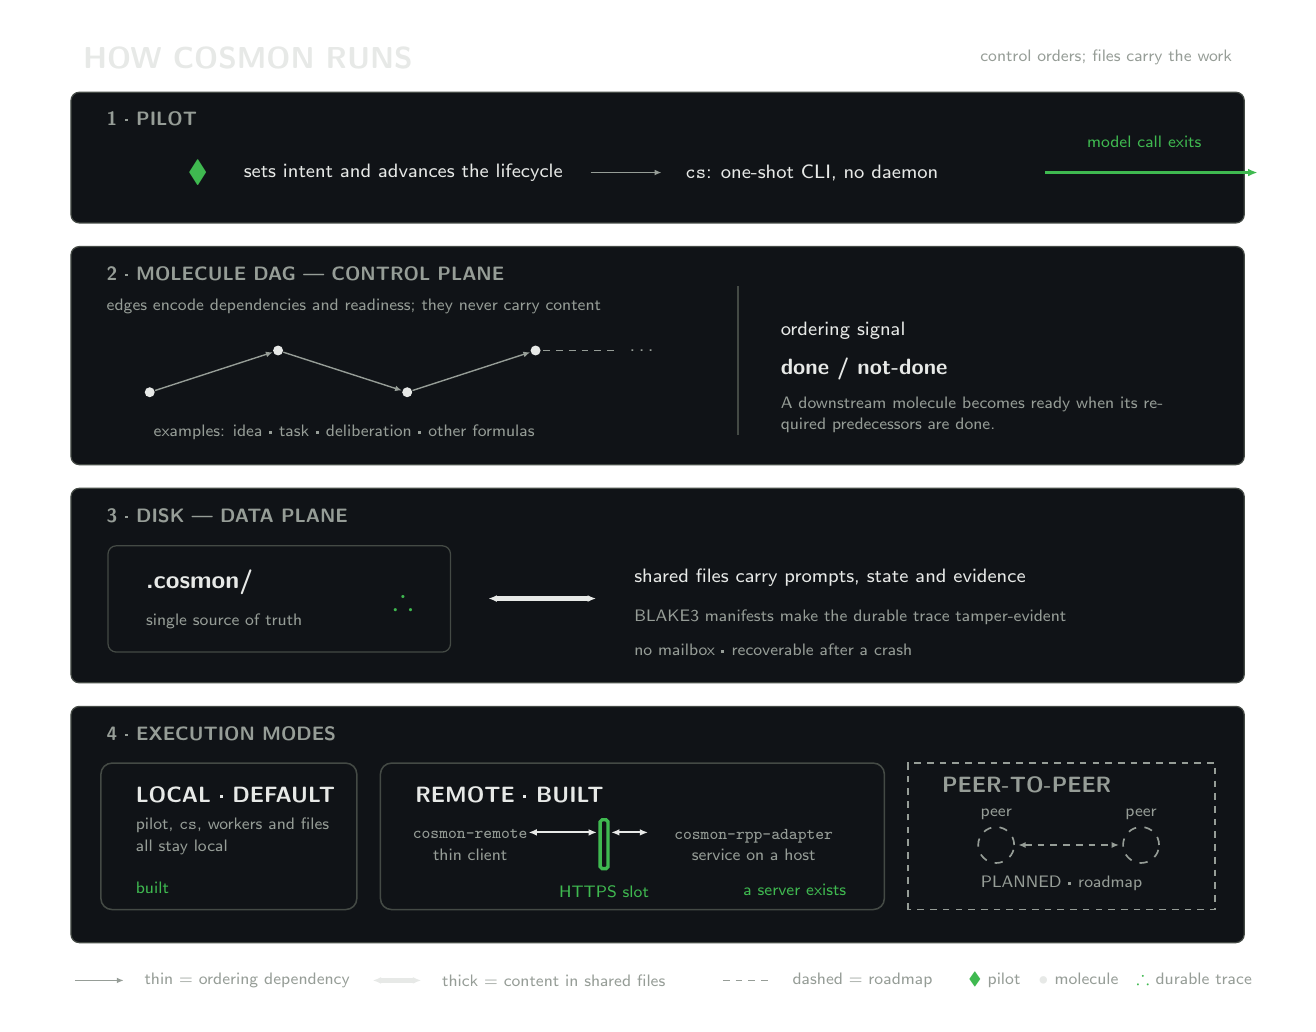
\begin{tikzpicture}[x=1cm,y=1cm]
  \useasboundingbox (0,0) rectangle (16,12.4);
  \node[cosmon title, anchor=west] at (.58,12.02) {HOW COSMON RUNS};
  \node[cosmon micro, anchor=east] at (15.42,12.02) {control orders; files carry the work};

  % 1 — pilot
  \draw[cosmon panel] (.55,9.92) rectangle (15.45,11.58);
  \node[cosmon label, anchor=west] at (.88,11.24) {1 · PILOT};
  \node[cosmon title] at (2.16,10.56) {\PilotGlyph};
  \node[cosmon small, anchor=west] at (2.62,10.56) {sets intent and advances the lifecycle};
  \draw[cosmon dependency] (7.15,10.56) -- (8.05,10.56);
  \node[cosmon small, anchor=west] at (8.23,10.56) {\texttt{cs}: one-shot CLI, no daemon};
  \draw[cosmon outbound] (12.92,10.56) -- (15.62,10.56);
  \node[cosmon micro, text=CosmonAccent, anchor=south] at (14.18,10.76) {model call exits};

  % 2 — DAG / control plane
  \draw[cosmon panel] (.55,6.85) rectangle (15.45,9.62);
  \node[cosmon label, anchor=west] at (.88,9.27) {2 · MOLECULE DAG — CONTROL PLANE};
  \node[cosmon micro, anchor=west] at (.88,8.86) {edges encode dependencies and readiness; they never carry content};

  \node[cosmon molecule] (m1) at (1.55,7.77) {};
  \node[cosmon molecule] (m2) at (3.18,8.30) {};
  \node[cosmon molecule] (m3) at (4.82,7.77) {};
  \node[cosmon molecule] (m4) at (6.45,8.30) {};
  \draw[cosmon dependency] (m1) -- (m2);
  \draw[cosmon dependency] (m2) -- (m3);
  \draw[cosmon dependency] (m3) -- (m4);
  \draw[cosmon roadmap] (6.55,8.30) -- (7.52,8.30);
  \node[cosmon small, text=CosmonMuted] at (7.82,8.30) {\ldots};
  \node[cosmon micro, anchor=north] at (4.02,7.48) {examples: idea · task · deliberation · other formulas};

  \draw[CosmonFaint, line width=.45pt] (9.02,7.23) -- (9.02,9.12);
  \node[cosmon small, anchor=west] at (9.44,8.55) {ordering signal};
  \node[cosmon small, font=\sffamily\bfseries\fontsize{8.2}{9.8}\selectfont, anchor=west]
    at (9.44,8.06) {done / not-done};
  \node[cosmon micro, anchor=west, text width=5.15cm] at (9.44,7.48)
    {A downstream molecule becomes ready when its required predecessors are done.};

  % 3 — disk / data plane
  \draw[cosmon panel] (.55,4.08) rectangle (15.45,6.55);
  \node[cosmon label, anchor=west] at (.88,6.20) {3 · DISK — DATA PLANE};
  \draw[cosmon panel] (1.02,4.47) rectangle (5.37,5.82);
  \node[cosmon small, font=\sffamily\bfseries\fontsize{9}{10.5}\selectfont, anchor=west]
    at (1.38,5.36) {.cosmon/};
  \node[cosmon micro, anchor=west] at (1.38,4.86) {single source of truth};
  \node[cosmon title, anchor=east] at (5.02,5.14) {\TraceGlyph};

  \draw[cosmon data] (5.85,5.15) -- (7.22,5.15);
  \node[cosmon small, anchor=west] at (7.58,5.42) {shared files carry prompts, state and evidence};
  \node[cosmon micro, anchor=west] at (7.58,4.91) {BLAKE3 manifests make the durable trace tamper-evident};
  \node[cosmon micro, anchor=west] at (7.58,4.50) {no mailbox · recoverable after a crash};

  % 4 — execution modes
  \draw[cosmon panel] (.55,.78) rectangle (15.45,3.78);
  \node[cosmon label, anchor=west] at (.88,3.43) {4 · EXECUTION MODES};

  \draw[cosmon frame] (.93,1.20) rectangle (4.18,3.06);
  \node[cosmon small, font=\sffamily\bfseries\fontsize{8}{9.5}\selectfont, anchor=west]
    at (1.25,2.66) {LOCAL · DEFAULT};
  \node[cosmon micro, anchor=west, text width=2.58cm] at (1.25,2.13)
    {pilot, \texttt{cs}, workers and files all stay local};
  \node[cosmon micro, text=CosmonAccent, anchor=west] at (1.25,1.48) {built};

  \draw[cosmon frame] (4.48,1.20) rectangle (10.88,3.06);
  \node[cosmon small, font=\sffamily\bfseries\fontsize{8}{9.5}\selectfont, anchor=west]
    at (4.80,2.66) {REMOTE · BUILT};
  \node[cosmon micro, anchor=center, align=center] (client) at (5.62,2.02)
    {\texttt{cosmon-remote}\\thin client};
  \draw[cosmon slot] (7.27,1.72) rectangle (7.37,2.34);
  \node[cosmon micro, text=CosmonAccent, anchor=north] at (7.32,1.62) {HTTPS slot};
  \node[cosmon micro, anchor=center, text width=2.52cm, align=center] (service) at (9.22,2.02)
    {\texttt{cosmon-rpp-adapter}\\service on a host};
  \draw[cosmon exchange] (6.36,2.18) -- (7.23,2.18);
  \draw[cosmon exchange] (7.41,2.18) -- (7.88,2.18);
  \node[cosmon micro, text=CosmonAccent, anchor=east] at (10.52,1.45) {a server exists};

  \draw[cosmon roadmap] (11.18,1.20) rectangle (15.08,3.06);
  \node[cosmon small, text=CosmonRoadmap, font=\sffamily\bfseries\fontsize{8}{9.5}\selectfont, anchor=west]
    at (11.49,2.78) {PEER-TO-PEER};
  \node[cosmon peer] (p1) at (12.30,2.02) {};
  \node[cosmon peer] (p2) at (14.14,2.02) {};
  \draw[cosmon roadmap arrow] (12.58,2.02) -- (13.86,2.02);
  \node[cosmon micro, text=CosmonRoadmap, anchor=south] at (12.30,2.22) {peer};
  \node[cosmon micro, text=CosmonRoadmap, anchor=south] at (14.14,2.22) {peer};
  \node[cosmon micro, text=CosmonRoadmap, anchor=south] at (13.13,1.32) {PLANNED · roadmap};

  \CosmonLegend
\end{tikzpicture}
\end{document}
